\documentclass[journal]{vgtc}                % final (journal style)

\usepackage{mathptmx}
\usepackage{graphicx}
\usepackage{times}
\usepackage{balance}
\usepackage{booktabs}
\usepackage{amsmath}
\usepackage[nooneline,hang,it,IT]{subfigure}
\usepackage{setspace}

% Slightly looser spacing to improve readability.
\setstretch{1.06}
\setlength{\parskip}{2pt}

\usepackage[bookmarks,backref=true,linkcolor=black]{hyperref}
\hypersetup{
  pdfauthor = {},
  pdftitle = {Expected Goals on Wyscout Open Data},
  colorlinks=true,
  linkcolor= black,
  citecolor= black,
  pageanchor=true,
  urlcolor = black,
  plainpages = false,
  linktocpage
}

\onlineid{0}
\vgtccategory{Research}
\vgtcinsertpkg

\title{Expected Goals on Public Football Data:\\
Logistic Regression vs.\ XGBoost}

\author{Zeyuan Sheng (zeysh403)}
\authorfooter{
\item
The author is with Link\"oping University, Sweden.
}

\abstract{
Expected Goals (xG) quantifies the quality of a shot by estimating the
probability that it results in a goal. Most publicly available xG models
rely on logistic regression, and I started this project fairly convinced
that a modern gradient-boosted tree model would do better. To check
this, I built a reproducible xG pipeline on the Wyscout open dataset
(45{,}246 shots from seven competitions) and compared logistic regression
with XGBoost, each combined with three strategies for handling class
imbalance. That did not happen: logistic regression is actually a little
ahead on this public feature set (AUC-ROC 0.771 against 0.764). I also
find that class weighting improves the threshold-dependent metrics while
barely changing the AUC, and that shot geometry together with the header
indicator dominate the feature importance.
}

\begin{document}

\maketitle

\section{Introduction}

Football is a low-scoring sport: a team can dominate a match, take twenty
shots, and still lose 1--0. The final goal count is therefore a noisy
measure of how well a team actually played. Expected Goals (xG) tries to
fix that by replacing the goal count with a sum of probabilities --- each
shot is assigned an estimated chance of being scored, and these are added
up over a match or a season. That total is usually more stable than the
raw goal count, which is why most data providers now publish some form of
xG.

The xG models available to the public, such as those on Understat or
FBref, are almost always logistic regressions over a small set of
geometric features. The more accurate models reported in the literature
generally depend on tracking data~\cite{xgSerieA2024}, which is not
something a student, or most clubs, can get hold of.

So the question I actually cared about is a practical one. If I am stuck
with public event data, is there anything to gain from swapping logistic
regression for a stronger model like XGBoost~\cite{chen2016xgboost}?
Alongside that, I wanted to see how much the usual class-imbalance
strategies really move the numbers, since that is rarely reported
side by side. All experiments use the Wyscout open
dataset~\cite{pappalardo2019wyscout}.

\section{Data and Method}

\subsection{Data}
The Wyscout dataset~\cite{pappalardo2019wyscout} covers the 2017/18
season of the five major European leagues together with the 2018 World
Cup and Euro 2016. From the full event stream I retained the shots and
free-kick shots and discarded penalties, since the xG of a penalty is
effectively a constant and would only add noise to the training data.
This leaves \textbf{45{,}246 shots}, of which roughly \textbf{10.2\%} are
goals. The goal rate varies little across the seven competitions (about
8--11\%), which matched what I expected for this kind of data.

Before training any model I plotted how conversion depends on distance and
angle (Figure~\ref{fig:eda}). Neither relationship is linear: the goal
rate falls sharply with distance and rises with the visible angle of the
goal. This lined up with what the model ended up using later.

\begin{figure*}[t]
\centering
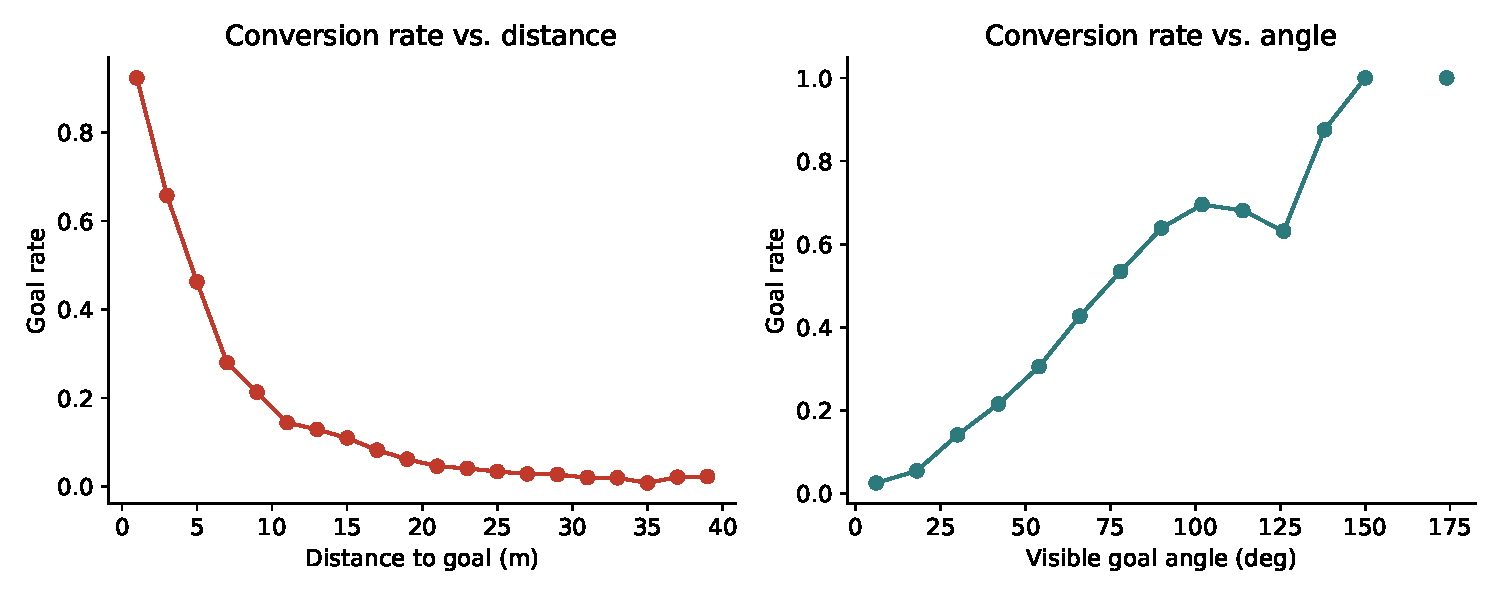
\includegraphics[width=0.85\textwidth]{figures/eda_distance_angle.pdf}
\caption{Empirical goal rate as a function of distance to goal (left)
and visible goal angle (right), computed on the full dataset.}
\label{fig:eda}
\end{figure*}

\subsection{Features}
Each shot is described by nine features. Four are geometric: the distance
to goal, the visible goal angle computed with Caley's
formula~\cite{caley2013xg}, and the raw $x,y$ position, which I retained
in case it captured information not already contained in the distance and
angle. Two are body-part indicators (foot, head), one marks free kicks,
and two describe the game state (the elapsed minute and the current score
difference).

\subsection{Models and the imbalance problem}
I compared two classifiers that are quite different in practice. Logistic
regression is the usual xG baseline: it is linear and its outputs can be
read as probabilities. XGBoost~\cite{chen2016xgboost} was the model I
expected to do better, since it picks up feature interactions on its own
and is often strong on tabular data. Putting them side by side was meant
to show whether the extra model complexity helped at all on this feature
set.

Goals are also rare ($\approx 10\%$). A model
that always predicts ``no goal'' is correct 90\% of the time yet is of no
practical use, so I paired each classifier with three standard imbalance
strategies: leaving the data unchanged, weighting the loss by inverse
class frequency, and oversampling the goals with
SMOTE~\cite{chawla2002smote}. SMOTE was fitted on the training fold only,
to avoid leakage. Two models and three strategies give the six
configurations reported below.

\subsection{Data split and evaluation}
I was careful to split the data by \emph{match} rather than by shot. If
two shots from the same game appear in both the training and test sets,
the model can exploit match-specific context, such as the lineups or the
run of play, and the test score becomes optimistic. I therefore split by
match: 70\% of matches for training, 15\% for validation and 15\% for test
(31{,}751 / 6{,}682 / 6{,}813 shots), with no match in more than one fold.
I report AUC-ROC and AUC-PR, which do not depend on the decision threshold,
together with F1, sensitivity and specificity at the usual 0.5 cut-off.
The pipeline is in Python
(\texttt{scikit-learn}, \texttt{xgboost}, \texttt{imbalanced-learn}) with
a fixed random seed.

\section{Results}

\subsection{Model comparison}
Table~\ref{tab:results} lists all six configurations, and the first thing
I noticed is that the comparison I built the whole project around did not
go the way I assumed. Logistic regression comes out ahead of XGBoost on
the threshold-free metrics in every single case: its best AUC-ROC is
0.771, against 0.764 for XGBoost. The gap is small, and I went back and
re-ran the split a few times half expecting it to flip, but it did not
--- the ordering held across all three imbalance strategies, so I do not
think it is just noise.

The imbalance strategy ended up mattering more than the model. Turning on
class weighting raises F1 from 0.17 to 0.32 and sensitivity from 0.10 to
roughly 0.68, while leaving the AUC essentially unchanged; in other
words, a usable decision threshold for almost nothing. SMOTE never
helped. It dragged XGBoost's AUC-ROC down from 0.764 to 0.755, and for
logistic regression it barely changed anything. So in practice, weighting
the loss seems like the safer choice than synthesising extra shots.

\begin{table}[t]
\centering
\caption{Test-set results (higher is better). Threshold $=0.5$ for
F1, sensitivity (Sens.) and specificity (Spec.).}
\label{tab:results}
\begin{tabular}{llrrrrr}
\toprule
Model & Imbalance & ROC & PR & F1 & Sens. & Spec. \\
\midrule
LR  & none         & 0.771 & 0.329 & 0.167 & 0.097 & 0.993 \\
LR  & class weight & 0.771 & 0.329 & 0.321 & 0.684 & 0.718 \\
LR  & SMOTE        & 0.771 & 0.328 & 0.321 & 0.672 & 0.725 \\
XGB & none         & 0.764 & 0.321 & 0.170 & 0.100 & 0.992 \\
XGB & class weight & 0.763 & 0.323 & 0.321 & 0.673 & 0.723 \\
XGB & SMOTE        & 0.755 & 0.310 & 0.334 & 0.333 & 0.928 \\
\bottomrule
\end{tabular}
\end{table}

Figure~\ref{fig:roc} shows the same pattern: all six curves sit almost on
top of each other, with the logistic-regression ones slightly ahead. I
would not have been able to rank them from the plot alone.

\begin{figure*}[t]
\centering
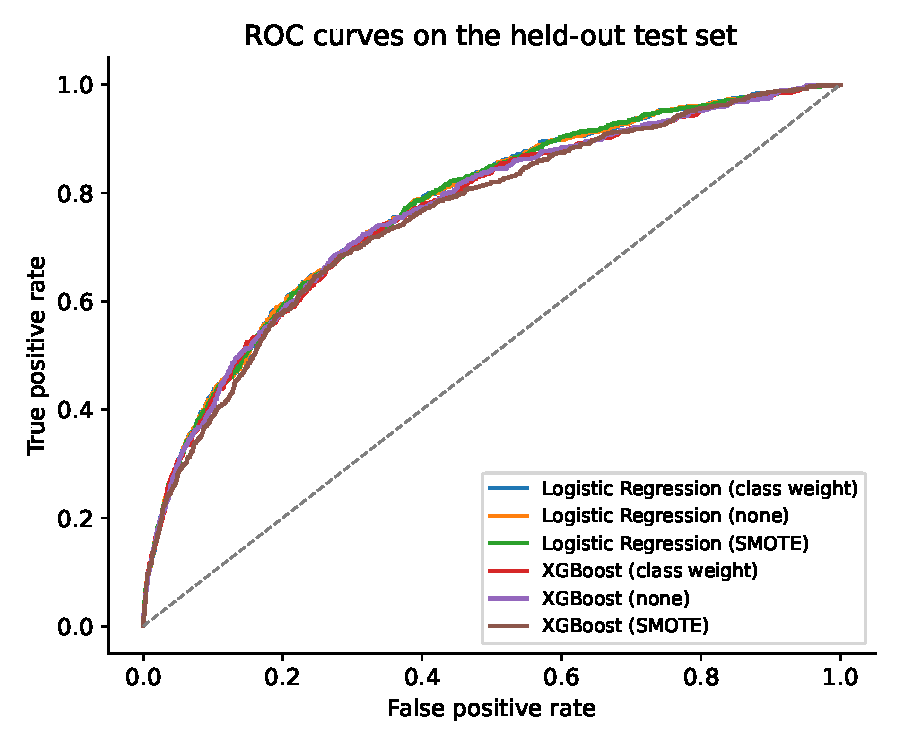
\includegraphics[width=0.62\textwidth]{figures/roc_curves.pdf}
\caption{ROC curves on the held-out test set. The dashed line is the
chance level. All six configurations are closely bunched.}
\label{fig:roc}
\end{figure*}

\subsection{Feature importance}
Figure~\ref{fig:fi} shows XGBoost's gain importances. I did not expect the
header indicator (\texttt{body\_head}) to rank first, ahead of
\texttt{angle}, \texttt{body\_foot}, and \texttt{distance}, but it makes
sense: a header from close range goes in far less often than a foot shot
from the same spot, so even after distance and angle are accounted for,
the body part still matters. The game-state and raw position features
barely show up.

\begin{figure}[t]
\centering
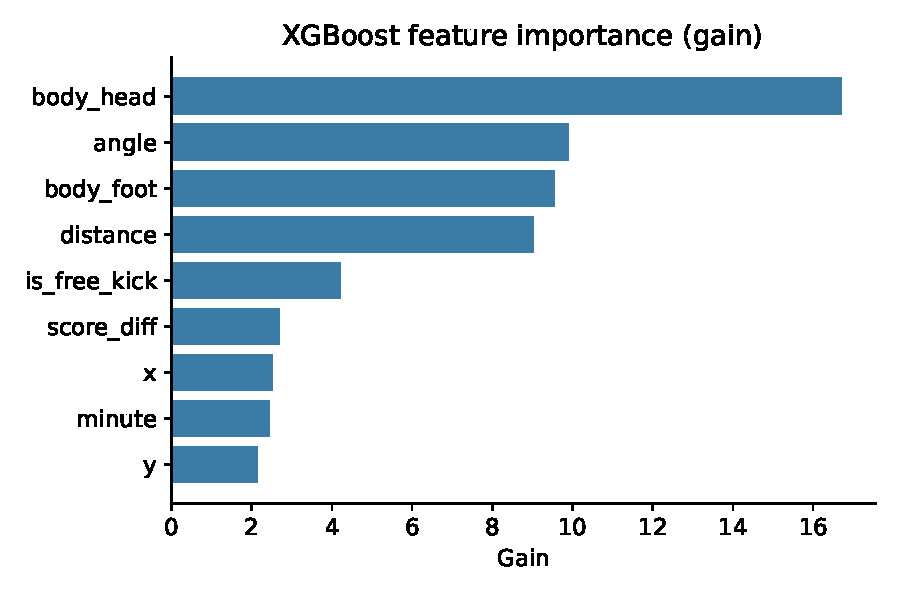
\includegraphics[width=\columnwidth]{figures/feature_importance.pdf}
\caption{XGBoost feature importance (gain). The head-shot indicator and
the geometric features dominate.}
\label{fig:fi}
\end{figure}

\section{Discussion}

So why doesn't XGBoost win? I am honestly not fully sure, but my best
explanation is that there just isn't much for it to exploit. The feature
set is small and mostly geometric, and once the features are scaled, the
relationship between distance and angle and the log-odds of a goal is
close to linear --- which is more or less the situation logistic
regression is built for. The bigger ensemble also has more room to
overfit on a dataset this size. Grinsztajn et al.~\cite{grinsztajn2022tabular}
report something similar on small tabular data, where linear models stay
competitive with tree ensembles, so I do not think this is only a quirk of
my setup. Still, I had expected at least a small edge from XGBoost, and
not getting one is the part of the project I am least settled about.

Cefis and Carpita~\cite{xgSerieA2024} report an AUC-ROC of about 0.79.
My best is 0.771, but they also use tracking data and a less conservative
split, so I would not make too much of the $\approx 0.02$ gap. Missing
defender and goalkeeper information, plus my match-level split, could
easily account for that difference. They also find that SMOTE loses to
simple class weighting, which matches what I saw.

There are clear limitations. There is no tracking data, only one season,
and Wyscout lumps several different shot situations together. The one I
care about most --- that I only measured how well the model \emph{ranks}
shots, not whether its probabilities are calibrated --- I come back to in
the conclusion.

\section{Conclusion}

Overall, the more complex model did not add much on this public xG setup.
Logistic regression matched XGBoost, class weighting was the imbalance
strategy worth using, and the model relied mainly on where the shot was
taken and whether it was a header.

If I had more time, I would check calibration next. This report only looks
at how well shots are ranked, but xG is a probability that gets summed up,
and a model can rank well while still giving biased probabilities. That
would feed into any season total, so it seems like the obvious next step,
and I did not get to it in this project.

\section{Implementation}
The code is in Python~3.11, using \texttt{pandas}, \texttt{scikit-learn},
\texttt{xgboost}, \texttt{imbalanced-learn}, and \texttt{matplotlib}. I
fixed the random seed (\texttt{RANDOM\_STATE = 42}) so the split and
metrics come out the same each run. The table and figures in this report
are generated from the saved model outputs, not copied by hand. The full
pipeline takes a few minutes on a laptop.

\bibliographystyle{abbrv}
\bibliography{refs}

\section*{Contributions from Each Project Member}\label{cont}

\begin{description}
\item[Zeyuan Sheng (zeysh403)] {All work: data preparation, feature
engineering, model training and evaluation, figures, and writing of
this report.}
\end{description}

\end{document}
